\section{Controls Introduction}
\hyperdef{ctrl}{introduction}{[Marker:ctrl.introduction]}\\
For the three main fields of detector controls, DAQ controls, and
board controls there are currently three products under test:
\begin{compactdesc}
\item[EPICS] Well known control system, widely used in accelarator
and classical controls. SNMP interface is available for monitoring
clusters and net devices. \item[LabView] Standard slow control at
GSI. \item[SysMES] Configuration control system developed at KIP.
Has CA interface to work with EPICS and SNMP. \item[xDAQ] DAQ
framework of CMS
\end{compactdesc}
Because it might be not possible to make a decision for one of
these to be used exclusively one should investigate/implement
interoperability. Communication standards in question:
\begin{compactitem}
\item DIM: DIM server in an EPICS IOC as first test bridge \item
CA: LabView CA client available \item SOAP: provided by xDAQ, Java
interface available.
\end{compactitem}
\begin{figure}[htb]
\centering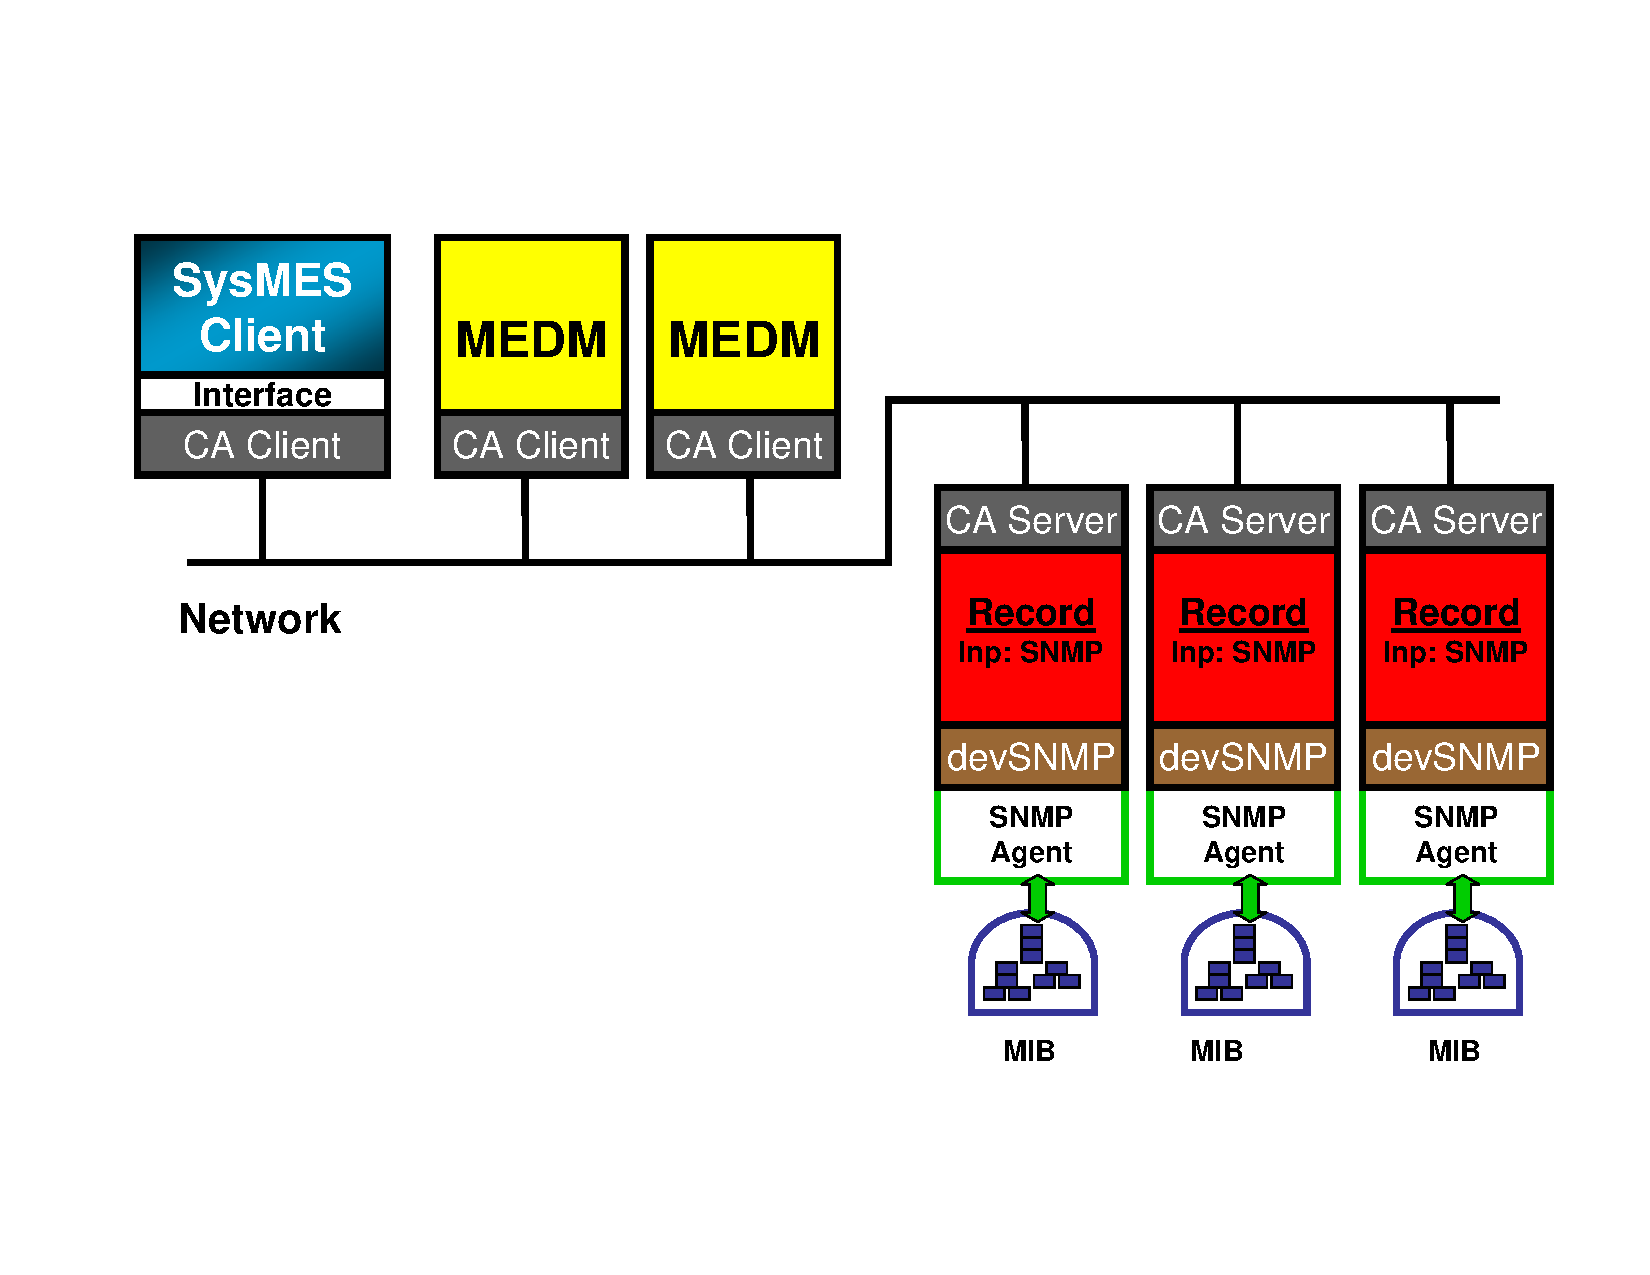
\includegraphics[width=.8\textwidth]
{demof-sysmes-epics-snmp} \caption{SNMP based control architecure}
\label{fig:sysmes-epics-snmp}
\end{figure}
The DAQ controls must provide the following functionality:
\begin{compactitem}
\item Control tasks on remote machines
\item Communicate with all tasks
\item Mechanism to store/retrieve the whole setup
\item Monitor setup, status, data flow, and performance
\item Control data flows
\item Visualization and GUI
\end{compactitem}
